\myChapter{3 ПРОВЕДЕННЫЕ ИССЛЕДОВАНИЯ. РЕЗУЛЬТАТЫ}
\vspace{-2em}
\section{3.1 Результаты тестирования}

Практически на всех задачах такие индексы как перебор и дерево квадрантов показали плохие результаты (рисунок 15), в свою очередь R-Tree и KD-Tree - основные финалисты. 
  \\
\begin{figure}[h]
    \centering
    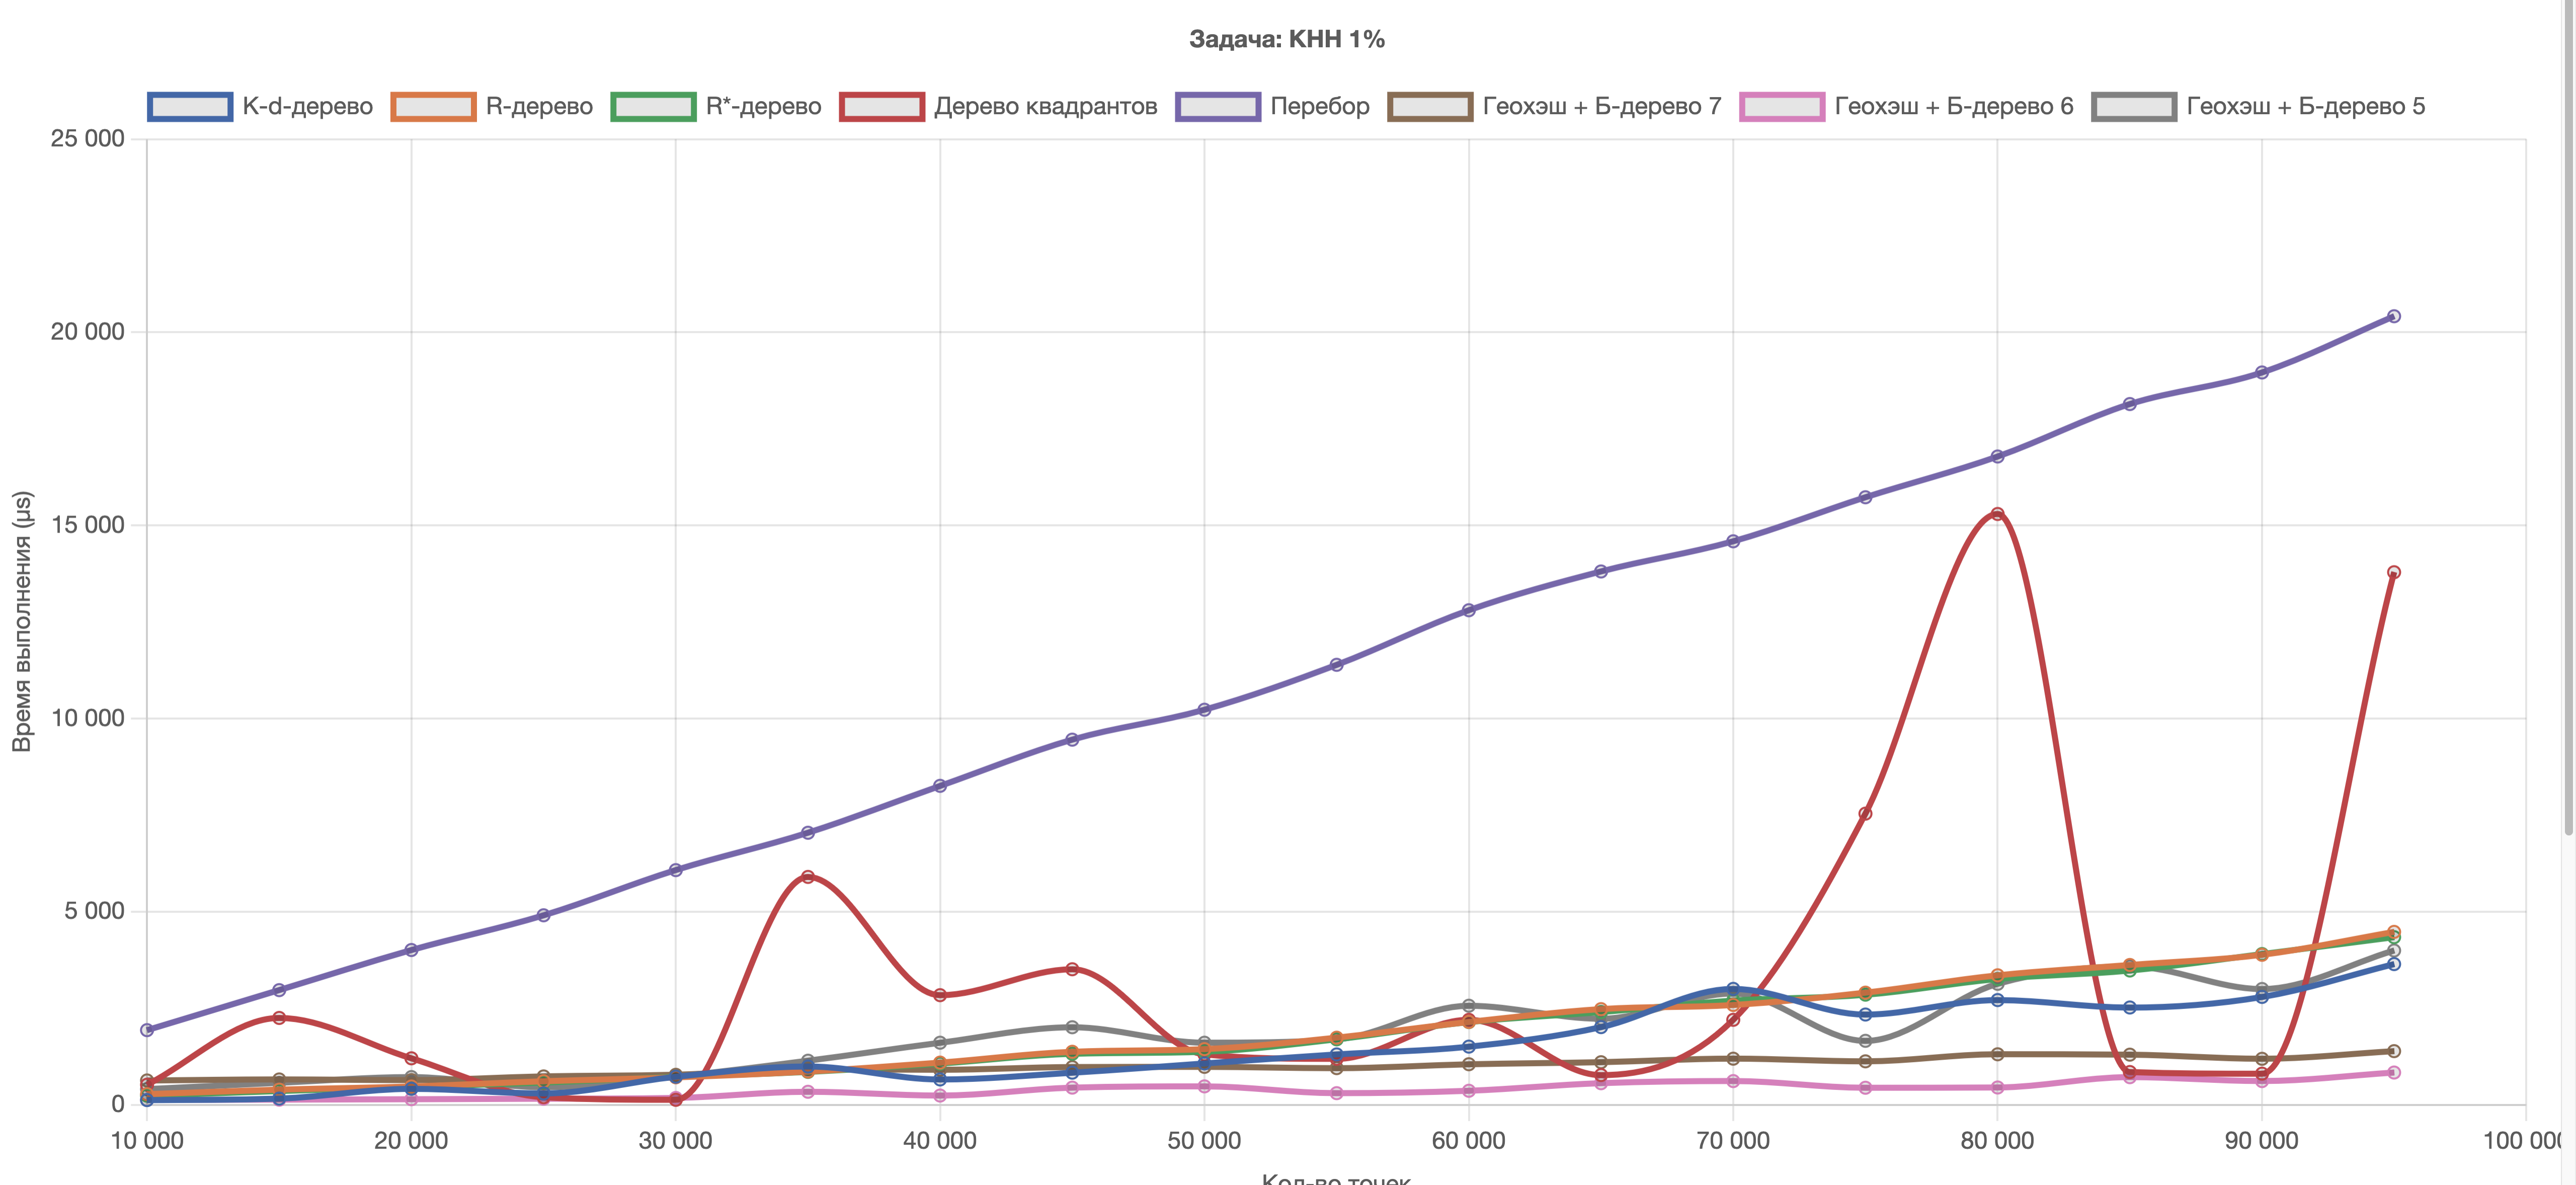
\includegraphics[scale=0.17]{results_knn_1.png}
    \caption{Задача KNN на 1\% точек}
\end{figure}

При этом разработанный индекс Geohash-B-Tree с правильной параметризацией всегда показывает крайне хорошие результаты (Рисунки 16 и 17).
\par\vspace{1em}
\begin{figure}[H]
    \centering
    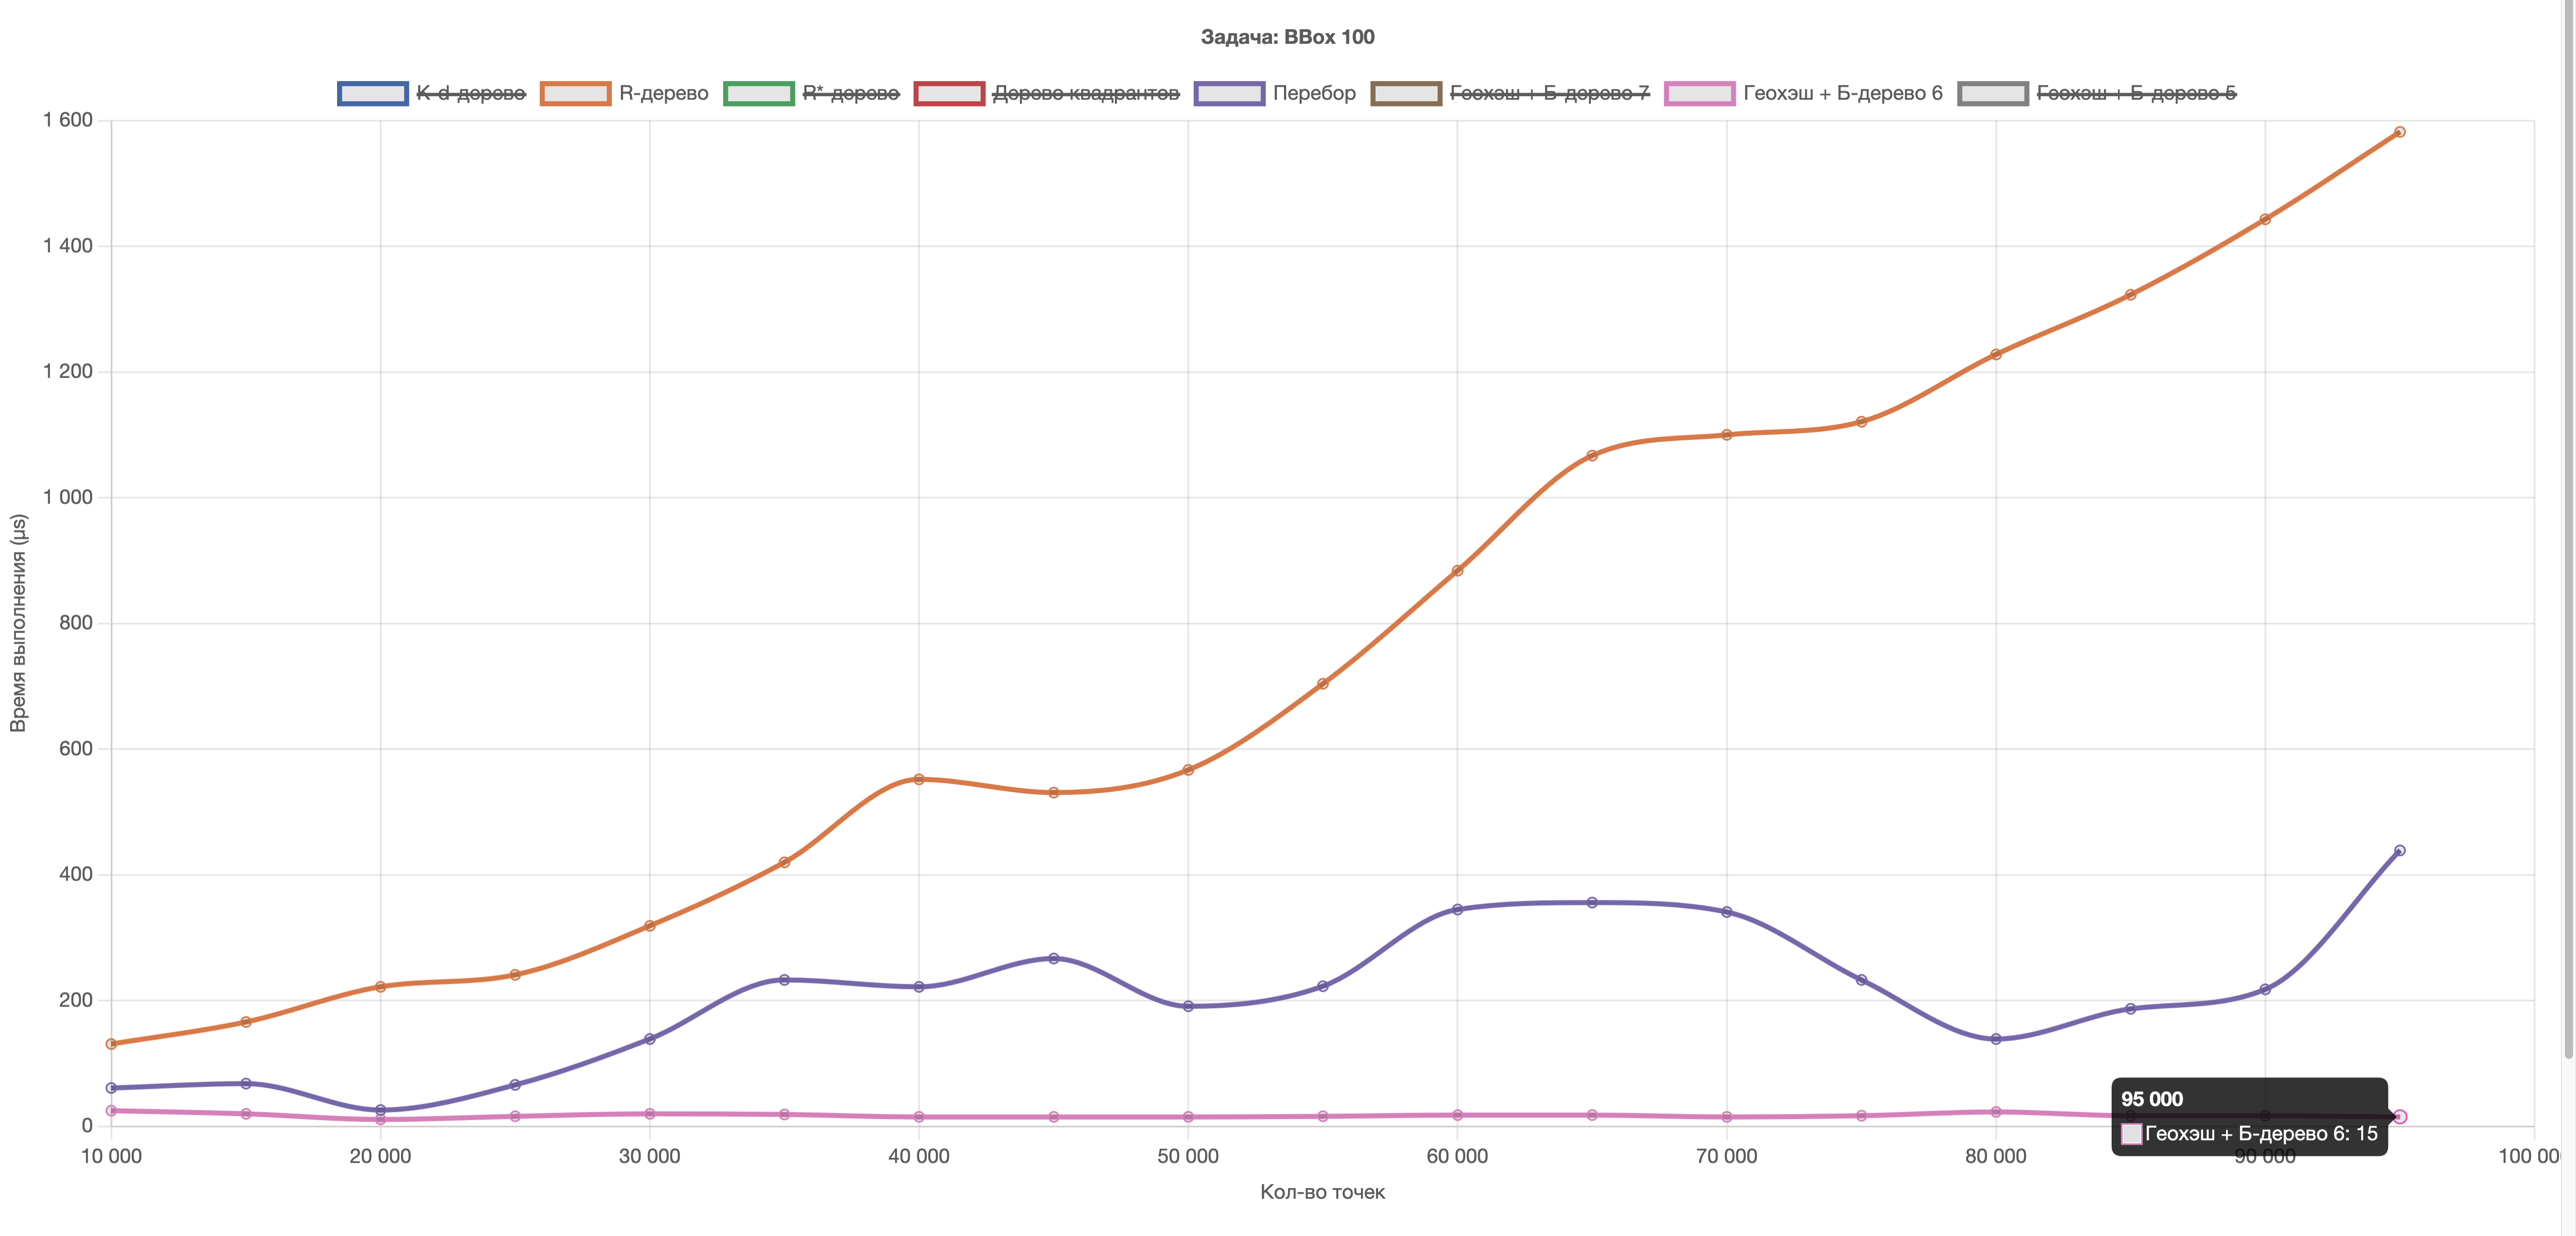
\includegraphics[scale=0.17]{results_bbox_100.png}
    \caption{Задача BBox на 100 случайных точках}
\end{figure}
\par\vspace{1em}
\begin{figure}[H]
    \centering
    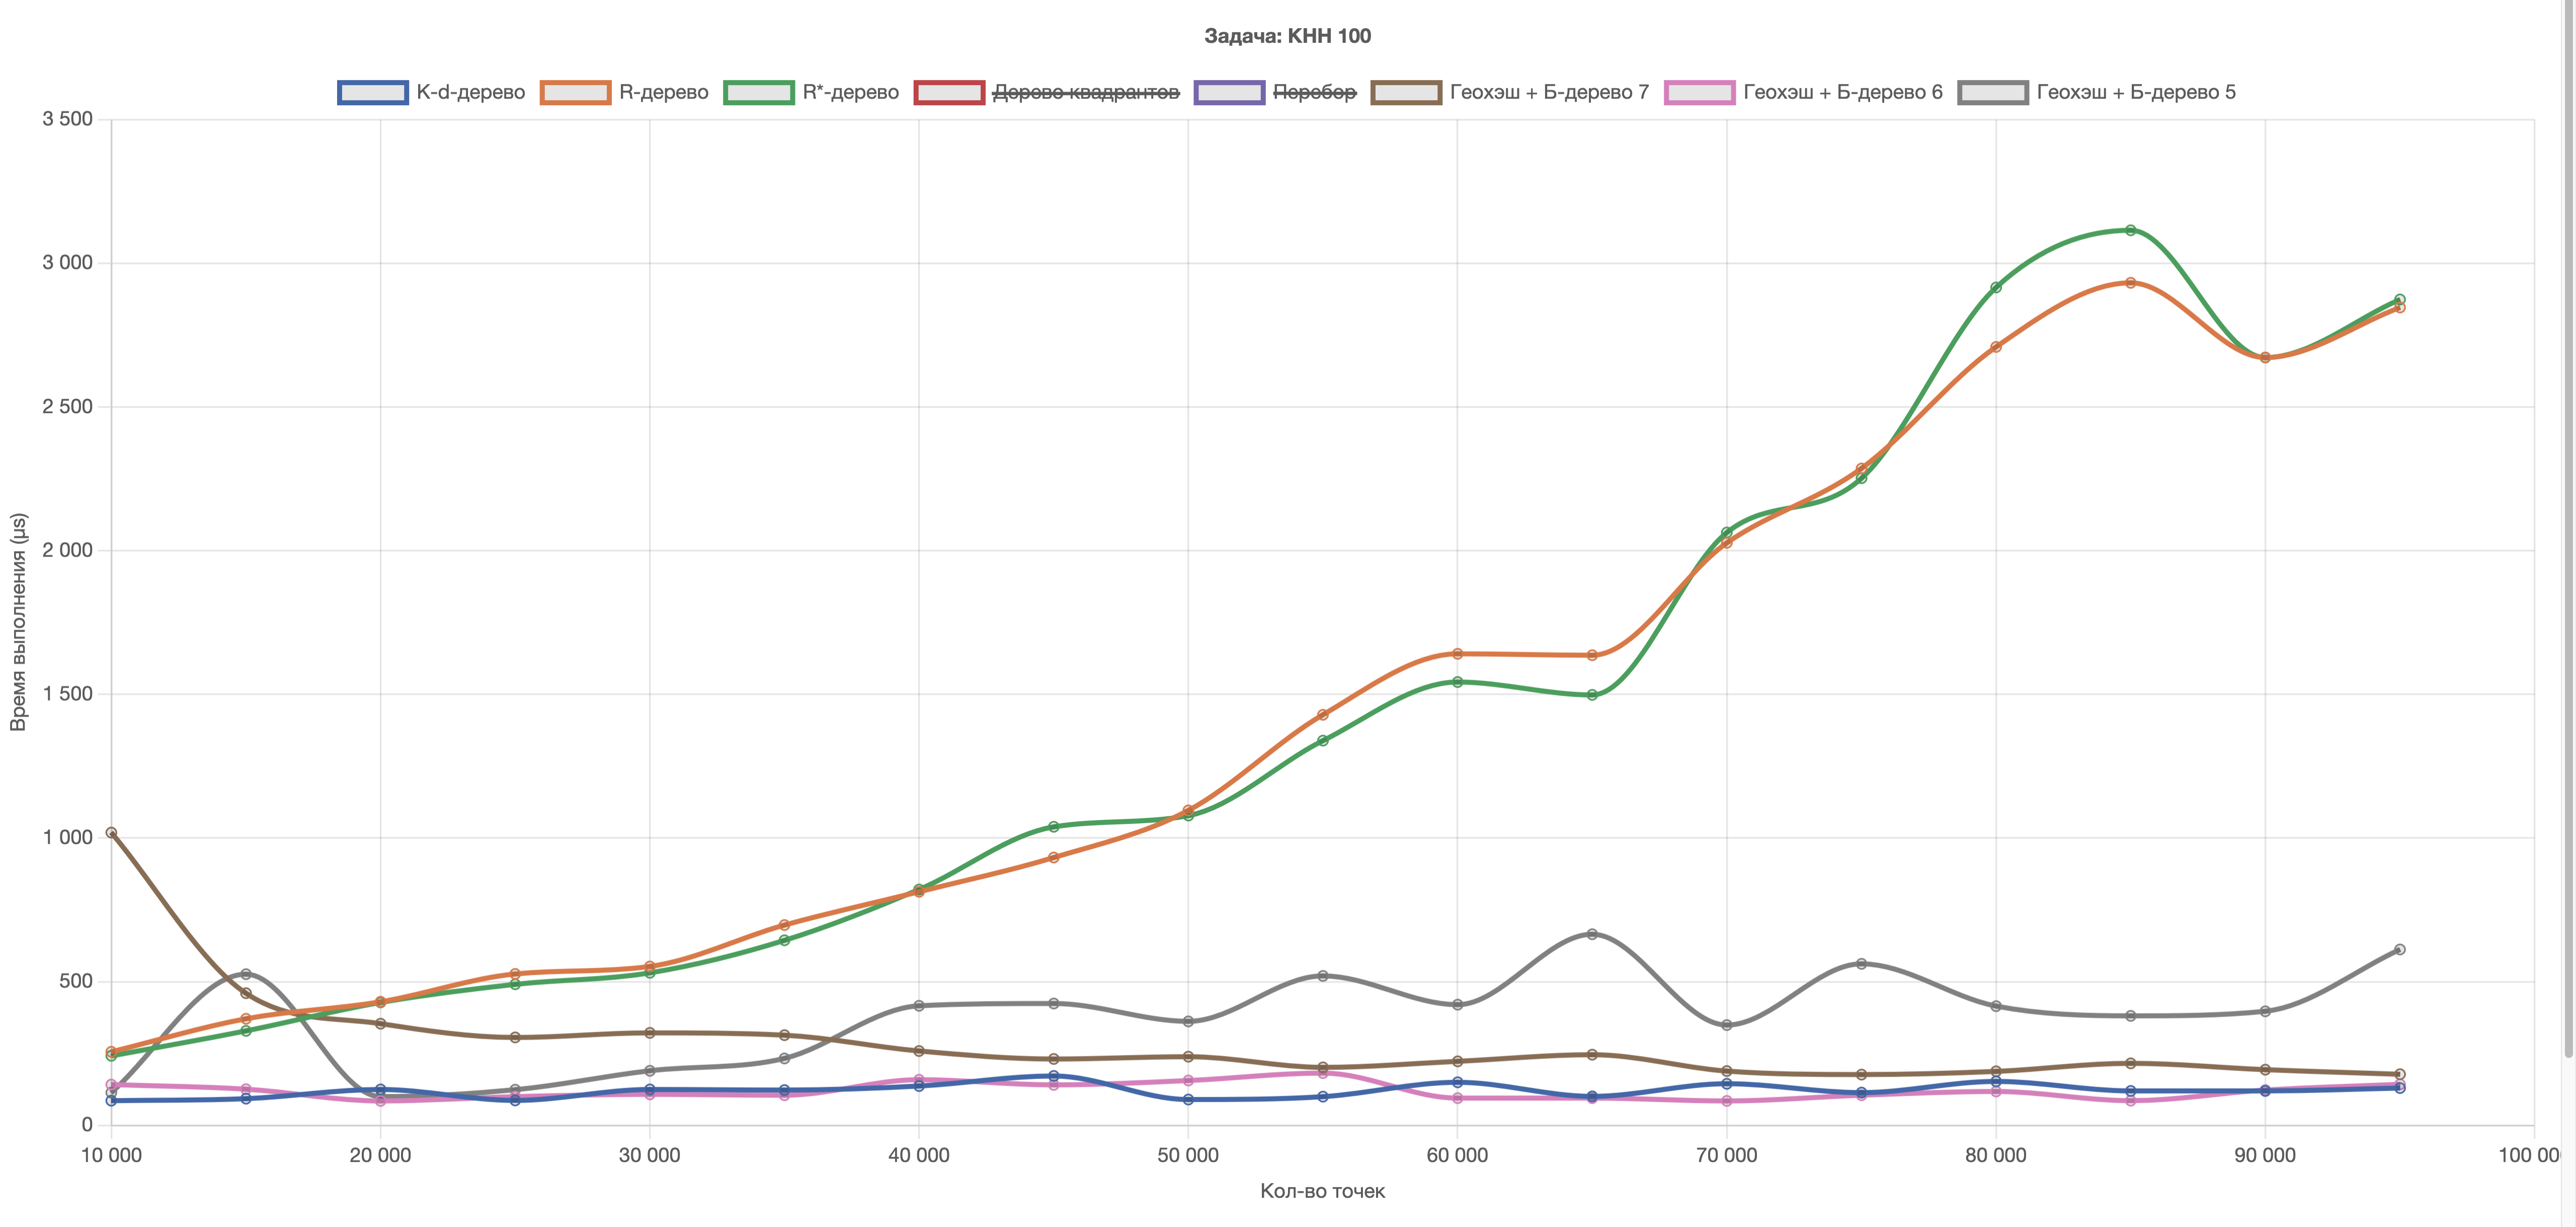
\includegraphics[scale=0.17]{results_knn_100.png}
    \caption{Задача KNN на 100 случайных точках}
\end{figure}
\par\vspace{1em}

\begin{samepage}
    Таким образом, можно сделать следующие выводы:
    \par а) популярные индексы R-Tree, KD-Tree и другие - в общем случае показывают крайне хорошие результаты;
    \par б) перебор часто работает быстрее, чем сложные индексы;
    \par в) разработанные индексы также показывают крайне хорошие результаты.
\end{samepage}

\section{3.2 Выводы}

По результатам проведенных работ, можно сделать следующие рекомендации относительно выбора индексов:
\par а) если используемая СУБД поддерживает геоиндексы - используйте их, например, из Redis, MongoDB и PostGIS;
\par б) если есть возможность выбрать индекс - рекомендуется выбрать индекс R-Tree, он имеет крайне большое количество методов, реализаций и в общем случае работает крайне хорошо;
\par в) если используемая СУБД не поддерживает геоиндексы - их можно реализовать через Geohash + B-Tree. Более сложные реализации (H3 + B-Tree, Geohash + R-Tree) тоже возможны, но не необходимы;
\par г) если требуется кластеризация, то для ключа кластерации можно использовать Geohash + B-Tree. Другие индексы не поддерживают кластеризацию.

\section{3.3 Результаты разработки системы тестирования}
Разработанное в ходе практической части программное обеспечение позволяет протестировать качество работы тех или иных индексов на разных задачах. Важно отметить, что полученное ПО является легко расширяемым, что позволяет разработчикам его использовать во время разработки, отладки и улучшения указанных индексов.

Преимуществами данной работы являются:
\par а) изолированность. Сервер исполнителя задач физически отделен от сервера менеджера;
\par б) наглядность. Пользователь в реальном времени видит результаты, может самостоятельно запрашивать задачи. 